\begin{figure}[t]
    \centering
    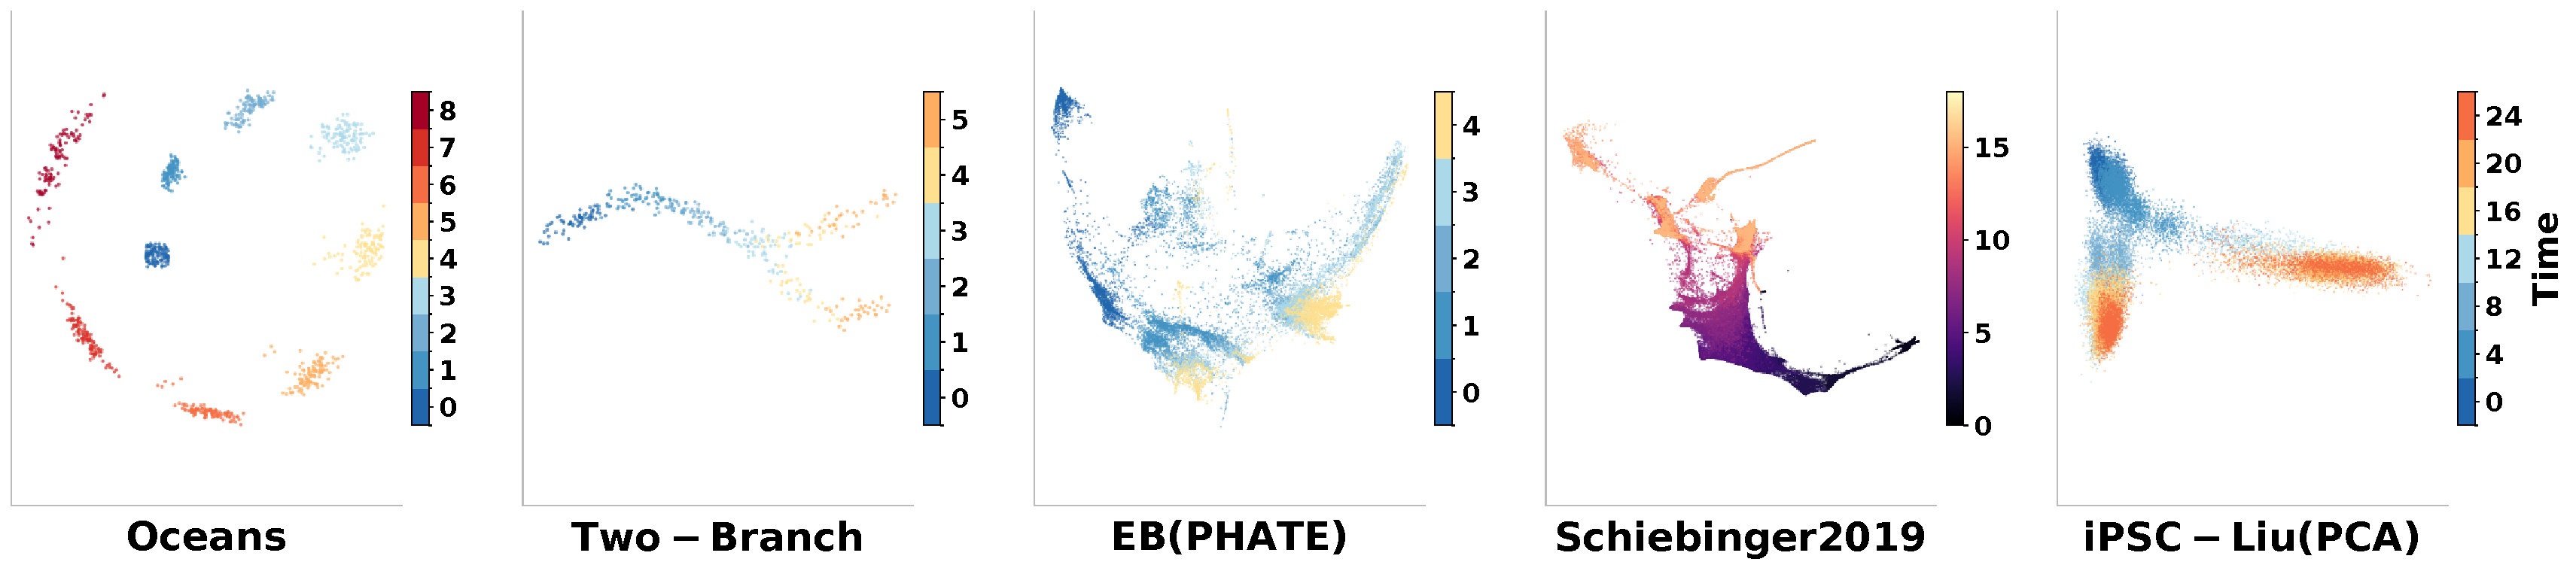
\includegraphics[width=0.88\linewidth]{figures/datasets_2d_overview.pdf} % PAGECUT: was 1.0\linewidth
    \caption{Overview of the 2D benchmark datasets. Points are colored by observed time for Ocean~\citep{petrovic2026curly}, Two-Branch, EB PHATE~\citep{moon2019visualizing}, Schiebinger2019~\citep{schiebinger2019optimal}, and iPSC-Liu~\citep{liu2020reprogramming}.}
    \label{fig:datasets-2d-overview}
\end{figure}
\begin{table}[hbtp]
\centering
\caption{Per-timepoint results on Ocean (2D)~\citep{petrovic2026curly}, holdout $t\in\{1,3,5,7\}$.}
\label{tab:ocean_2d_1_3_5_7}
\small
\setlength{\tabcolsep}{4pt}
\resizebox{1\linewidth}{!}{
\begin{tabular}{lcccccccccccc}
\toprule
Method & \multicolumn{4}{c}{MMD $\downarrow$} & \multicolumn{4}{c}{$\mathcal{W}_1\downarrow$} & \multicolumn{4}{c}{$\mathcal{W}_2\downarrow$} \\
\cmidrule(lr){2-5} \cmidrule(lr){6-9} \cmidrule(lr){10-13}
 & $t=1$ & $t=3$ & $t=5$ & $t=7$ & $t=1$ & $t=3$ & $t=5$ & $t=7$ & $t=1$ & $t=3$ & $t=5$ & $t=7$ \\
\midrule
Action Matching & \underline{0.7429} & 1.0662 & 0.9465 & 1.1289 & 0.3549 & 0.4823 & 0.2383 & 0.5073 & 0.3662 & 0.4846 & 0.2425 & 0.5143 \\
Aligned CFM & 0.7989 & 0.8754 & 1.0073 & 0.8272 & 0.0976 & 0.1644 & 0.3024 & 0.2245 & 0.1017 & 0.1673 & 0.3046 & 0.2262 \\
CURLY & 1.0545 & 0.8373 & 0.5869 & 0.8663 & 0.3766 & 0.1521 & 0.1077 & 0.2638 & 0.3771 & 0.1537 & 0.1102 & 0.2646 \\
DMSB & 1.1260 & \underline{0.6089} & \underline{0.2542} & \underline{0.4962} & 0.3060 & \underline{0.1097} & \underline{0.0435} & \underline{0.1097} & 0.3065 & \underline{0.1150} & \underline{0.0473} & \underline{0.1142} \\
MFM & 0.8482 & 0.7859 & 0.6928 & 0.5823 & \underline{0.0960} & 0.1433 & 0.1359 & 0.1279 & \underline{0.0991} & 0.1452 & 0.1385 & 0.1302 \\
OT-CFM & 0.9410 & 0.8169 & 0.6827 & 0.6305 & 0.1227 & 0.1428 & 0.1289 & 0.1321 & 0.1255 & 0.1459 & 0.1308 & 0.1334 \\
\midrule
\textbf{\model (ours)} & \textbf{0.4504} & \textbf{0.2588} & \textbf{0.0735} & \textbf{0.2779} & \textbf{0.0399} & \textbf{0.0398} & \textbf{0.0268} & \textbf{0.0505} & \textbf{0.0440} & \textbf{0.0434} & \textbf{0.0362} & \textbf{0.0534} \\
\bottomrule
\end{tabular}
}
\end{table}

\section{Experiment}
\label{sec:experiment}
The experiments evaluate PACE through five questions. First, on controlled 2D trajectories, can PACE recover smooth and branching geometry without paired identities or velocity supervision (Figure~\ref{fig:datasets-2d-overview}; Tables~\ref{tab:ocean_2d_1_3_5_7} and~\ref{tab:branch_toy_dim2})? Second, when reference velocities are available only for evaluation, do the learned dynamics align with held-out velocity fields on Ocean and EB PHATE (Figure~\ref{fig:velocity-diagnostics}; Appendix Tables~\ref{tab:ocean_holdout_velocity_metrics} and~\ref{tab:ebphate_holdout_velocity_metrics})? Third, on biological time courses, does PACE improve held-out reconstruction for single-cell differentiation and reprogramming from destructive snapshots (Table~\ref{tab:single_cell_2d_time_average})? Fourth, does PACE remain effective as the representation dimension increases (Tables~\ref{tab:ipsc_liu_dim10_50_mean})? Finally, which components of PACE account for the observed gains (Figure~\ref{fig:pace-ablation-per-tp})?
\subsection{Experimental setup}

\textbf{Evaluation protocol. }
All experiments use the same held-out snapshot protocol: methods observe only the training time points and are evaluated on the held-out time points listed in each table caption. We report distributional reconstruction quality using maximum mean discrepancy (MMD), 1-Wasserstein distance ($\mathcal{W}_1$), and 2-Wasserstein distance ($\mathcal{W}_2$); lower is better, bold denotes the best result, and underline denotes the second best.

\textbf{Datasets. }
Our benchmark suite includes controlled 2D temporal point clouds and biological single-cell time-course datasets.
The controlled datasets are designed to isolate geometric behavior in low-dimensional temporal data, including Ocean~\citep{shen2025multimarginal,petrovic2026curly} and a branching toy dataset, without relying on cell identities or velocity supervision.
The biological datasets test destructive snapshot settings in which individual cell identities are not shared across time, covering embryoid body differentiation~\citep{moon2019visualizing}, mouse reprogramming~\citep{schiebinger2019optimal}, induced trophoblast stem-cell reprogramming~\citep{liu2020reprogramming}, and multimodal CITE-seq/Multiome time courses~\citep{lance2022multimodal}.
% PAGECUT: merged two sentences into one (originals below) for the ICLR page limit.
% Figure~\ref{fig:datasets-2d-overview} gives a visual overview of the 2D datasets used in the main low-dimensional experiments.
% Detailed dataset sources and preprocessing choices are provided in Appendix~\ref{sec:app:benchmarks}.
Figure~\ref{fig:datasets-2d-overview} visualizes the 2D datasets; dataset sources and preprocessing are in Appendix~\ref{sec:app:benchmarks}.

\textbf{Baselines. }
We compare against representative transport- and flow-based trajectory models, covering action-based continuous dynamics~\citep{neklyudov2023action}, minibatch optimal-transport flow matching~\citep{tong2023conditional}, metric/geodesic flow matching~\citep{kapusniak2024metric}, pseudo-velocity-corrected flows~\citep{petrovic2026curly}, adversarial multi-marginal interpolant learning~\citep{kviman2026multimarginal}, and stochastic Schr\"odinger bridge dynamics~\citep{chen2023deep}.
Implementation details for baselines and PACE are provided in Appendices~\ref{sec:app:baselines} and~\ref{sec:app:pace-implementation}.
Qualitative prediction-versus-held-out overlays for the same 2D runs are shown in Appendix Figures~\ref{fig:app:stage2-ocean}--\ref{fig:app:stage2-ipsc}.



\subsection{Controlled 2D trajectories}

\begin{figure}[htp]
    \centering
    \begin{minipage}[t]{0.455\linewidth} % PAGECUT: was 0.49\linewidth
        \centering
        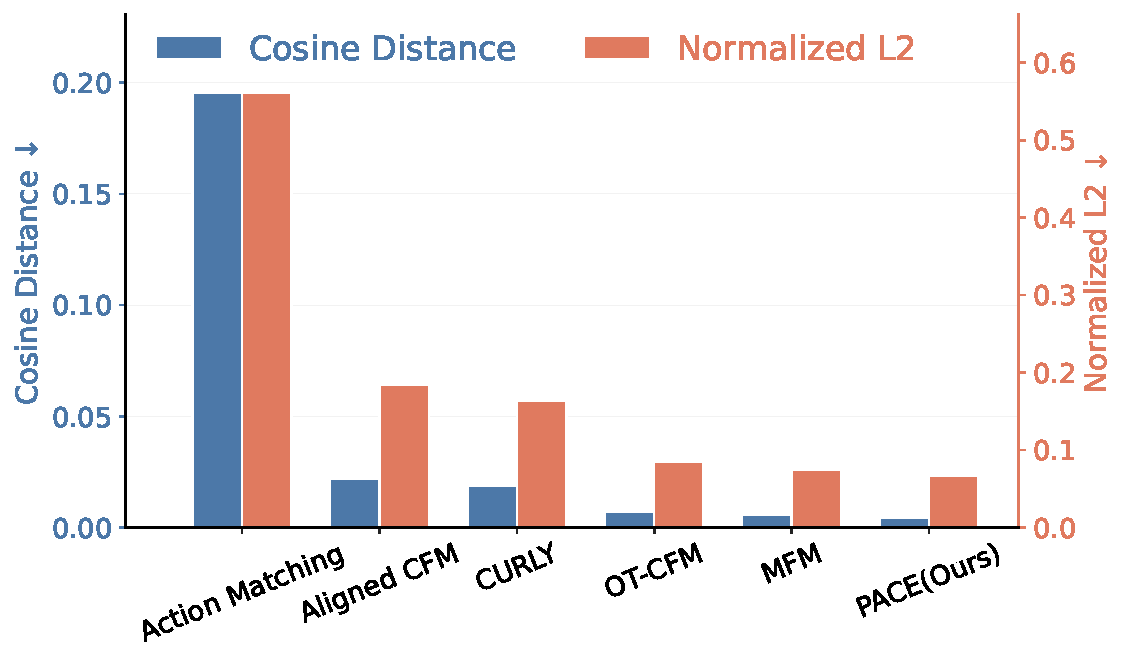
\includegraphics[width=\linewidth]{figures/ocean_velocity.pdf}
        \centerline{\small (a) Ocean}
    \end{minipage}\hfill
    \begin{minipage}[t]{0.455\linewidth} % PAGECUT: was 0.49\linewidth
        \centering
        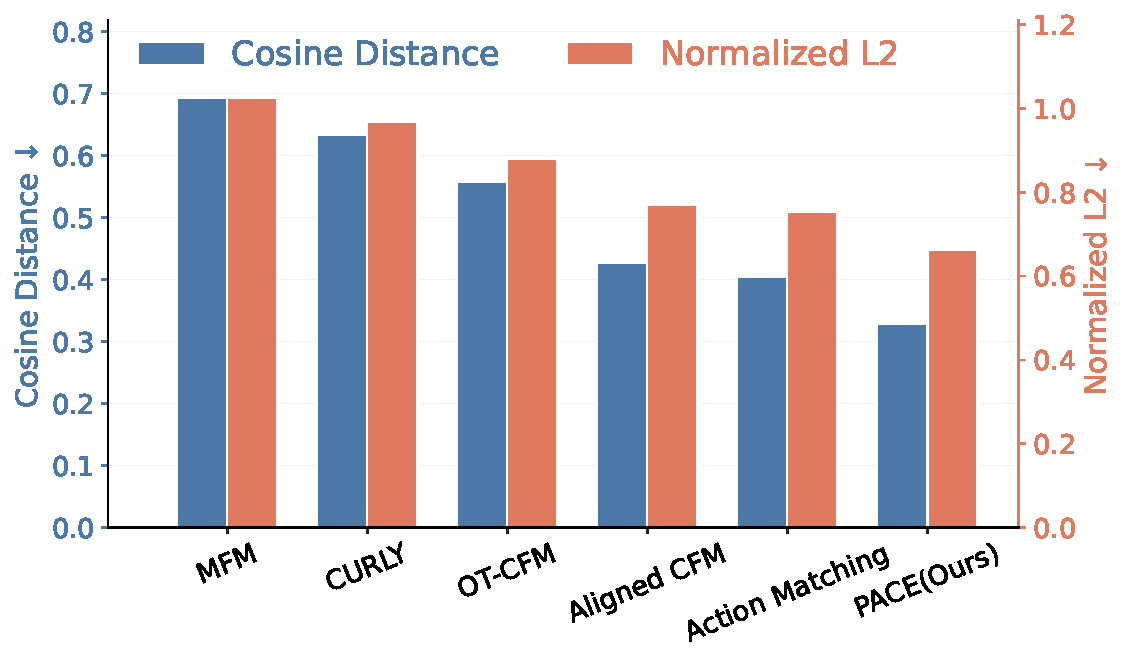
\includegraphics[width=\linewidth]{figures/eb_phate_velocity.pdf}
        \centerline{\small (b) EB PHATE}
    \end{minipage}
    % PAGECUT: caption compressed for the ICLR page limit. Original:
    % "Velocity-alignment diagnostics on Ocean and EB PHATE. Ocean compares learned velocities with held-out simulator velocities, while EB PHATE compares learned 2D velocities with the RNA-velocity reference. Bars report cosine distance and normalized L2 error; lower is better."
    \caption{Velocity-alignment diagnostics on Ocean~\citep{petrovic2026curly} and EB PHATE~\citep{moon2019visualizing}, comparing learned velocities with held-out simulator velocities (Ocean) or the RNA-velocity reference (EB PHATE). Bars report cosine distance and normalized $L_2$ error; lower is better. }
    \label{fig:velocity-diagnostics} 
\end{figure}

We evaluate PACE on two controlled 2D settings, including Ocean, a rotational non-gradient benchmark from Curly Flow Matching~\citep{petrovic2026curly}, and a Two-Branch toy benchmark. Methods observe only unpaired point positions; simulator velocities and latent identities are not used for training.
For Ocean, we also hold out evaluation snapshots and compare the learned velocity field at those times with the simulator velocity field, testing whether the inferred dynamics recover the correct directionality rather than only matching held-out marginals.

Tables~\ref{tab:ocean_2d_1_3_5_7} and~\ref{tab:branch_toy_dim2} show that PACE gives the strongest overall held-out reconstruction. It is best on all Ocean metrics and remains strongest on most Two-Branch entries, with CURLY slightly better only for late-branch $\mathcal{W}_2$. The Ocean panel in Figure~\ref{fig:velocity-diagnostics} further checks the learned velocity direction against held-out simulator velocities; the per-timepoint diagnostic values are reported in Appendix Table~\ref{tab:ocean_holdout_velocity_metrics}. Together, these results indicate that the geometry-aware bias helps recover both smooth rotational motion and simple branching structure from snapshots alone.

\subsection{Low-dimensional single-cell trajectories}

We next ask whether the same behavior carries over to biological time courses represented in low-dimensional embeddings, where the true cell identities are unobserved and geometric structure must be inferred from destructive snapshots. 
Table~\ref{tab:single_cell_2d_time_average} summarizes the time-averaged low-dimensional biological results across EB PHATE, iPSC-Liu, and Schiebinger2019; the corresponding per-timepoint results are reported in Appendix Tables~\ref{tab:eb_phate_2d_3}, \ref{tab:ipsc_liu_2d_4_16}, and~\ref{tab:schiebinger2019_2d_6_11_16}. On EB PHATE, PACE obtains the best MMD, $\mathcal{W}_1$, and $\mathcal{W}_2$, showing that the method improves held-out marginal reconstruction in a manifold-aware PHATE embedding. The EB PHATE panel in Figure~\ref{fig:velocity-diagnostics} adds an independent directionality check by comparing the learned 2D velocity field at the held-out snapshot with RNA velocity, which is used only for evaluation. Appendix Table~\ref{tab:ebphate_holdout_velocity_metrics} 
shows that PACE also best aligns with this external velocity proxy, 
suggesting that the gain reflects both endpoint reconstruction and plausible local flow direction. 
On iPSC-Liu 2D, PACE is best on every reported metric. 
On Schiebinger2019, PACE is best on seven of nine detailed metric-timepoint entries and remains close on the remaining final-time scores. 
% PAGECUT: removed redundant summary sentence for the ICLR page limit:
% "Overall, the low-dimensional biological results show that PACE transfers the controlled-geometry gains to both differentiation and reprogramming snapshots."
Compared with the strongest baseline for each dataset--metric pair, PACE reduces MMD, $\mathcal{W}_1$, and $\mathcal{W}_2$ by 36.2\%, 21.5\%, and 13.6\% on EB PHATE; by 16.1\%, 26.4\%, and 25.0\% on iPSC-Liu; and by 31.2\%, 25.5\%, and 22.4\% on Schiebinger2019.

\begin{table}[!htbp]
\centering
\scriptsize
\setlength{\tabcolsep}{3pt}
\renewcommand{\arraystretch}{0.88}
\caption{Time-averaged low-dimensional single-cell results. EB~\citep{moon2019visualizing} uses $t=3$, iPSC-Liu~\citep{liu2020reprogramming} uses $t\in\{4,16\}$, and Schiebinger2019~\citep{schiebinger2019optimal} uses $t\in\{6,11,16\}$.}
\label{tab:single_cell_2d_time_average}
\resizebox{\linewidth}{!}{
\begin{tabular}{lccccccccc}
\toprule
Method
& \multicolumn{3}{c}{EB PHATE}
& \multicolumn{3}{c}{iPSC-Liu}
& \multicolumn{3}{c}{Schiebinger2019} \\
\cmidrule(lr){2-4} \cmidrule(lr){5-7} \cmidrule(lr){8-10}
& MMD $\downarrow$ & $\mathcal{W}_1\downarrow$ & $\mathcal{W}_2\downarrow$
& MMD $\downarrow$ & $\mathcal{W}_1\downarrow$ & $\mathcal{W}_2\downarrow$
& MMD $\downarrow$ & $\mathcal{W}_1\downarrow$ & $\mathcal{W}_2\downarrow$ \\
\midrule
Action Matching
& 0.2436 & 0.4553 & 0.5273
& 0.5230 & 0.8005 & 0.9730
& 0.4057 & 0.4161 & 0.4754 \\
Aligned CFM
& \underline{0.1056} & \underline{0.2657} & \underline{0.3243}
& 0.5428 & \underline{0.6594} & \underline{0.8320}
& 0.3239 & 0.3175 & 0.3931 \\
CURLY
& 0.1384 & 0.3223 & 0.4422
& 0.5613 & 0.7186 & 0.9216
& 0.7687 & 1.3684 & 1.4660 \\
DMSB
& 0.1325 & 0.3053 & 0.4341
& 0.6456 & 1.0244 & 1.1023
& \underline{0.3030} & \underline{0.2774} & \underline{0.3662} \\
MFM
& 0.1518 & 0.3704 & 0.4451
& 0.5533 & 0.6657 & 0.8838
& 0.6990 & 1.5897 & 1.7942 \\
OT-CFM
& 0.1069 & 0.2784 & 0.3622
& \underline{0.5228} & 0.7166 & 0.9261
& 0.8072 & 1.9095 & 2.0235 \\
\midrule
\textbf{\model (ours)}
& \textbf{0.0674} & \textbf{0.2087} & \textbf{0.2803}
& \textbf{0.4385} & \textbf{0.4853} & \textbf{0.6238}
& \textbf{0.2084} & \textbf{0.2067} & \textbf{0.2840} \\
\bottomrule
\end{tabular}
}
\end{table}


% PAGECUT: removed the manual \newpage that preceded this subsection in the
% NeurIPS layout; it pins Sec.~4.4 to a fresh page and wastes space in ICLR layout.
\subsection{Higher-dimensional single-cell benchmarks}

% PAGECUT: this subsection was a two-minipage block (text 0.53 + Table 3 at 0.44\linewidth).
% The table moved to Appendix~\ref{sec:app:concentration} as Table~\ref{tab:ipsc_liu_dim10_50_mean};
% the text below is unchanged and now spans the full line width.
High-dimensional PCA tests whether PACE still helps when Euclidean distances lose temporal contrast. On iPSC-Liu, PACE is best on all time-averaged 10D/50D metrics in Table~\ref{tab:ipsc_liu_dim10_50_mean}. On OP-Cite/OP-Multi 100D, it remains on the empirical Pareto front, leading OP-Cite MMD and OP-Multi $\mathcal{W}_1/\mathcal{W}_2$ in Appendix Table~\ref{tab:op_100d}. Figure~\ref{fig:norm-time-concentration-vs-dim} shows the diagnostic behind this regime, with norm CV approaching $0.3$ and inter-time separation approaching the within-time radius. The useful signal is therefore not global separation between time means, but local anisotropy within each snapshot; PACE turns that local geometry into coupling costs. This helps distinguish directionally consistent moves from distance-similar but geometrically implausible pairings. Appendix~\ref{sec:app:concentration} and Figures~\ref{fig:app:ipsc_dim}--\ref{fig:app:ipsc} provide the detailed concentration analysis.


\subsection{Ablation study}

% PAGECUT: ablation paragraph tightened for the ICLR 9-page limit. Original:
% We finally isolate the contribution of the main PACE components on the Schiebinger2019 holdouts used in Table~\ref{tab:schiebinger2019_2d_6_11_16}. Figure~\ref{fig:pace-ablation-per-tp} compares the full model with variants that remove coupling rematching, set the metric penalty to the Euclidean case, use all neighbors rather than local neighborhoods, or ablate the spatial and temporal kernel structure used to smooth local geometry. Each simplification degrades at least one metric or time point, and the full PACE variant gives the most stable low errors across MMD, W1, and W2. This indicates that the gains do not come from a single implementation detail: the anisotropic metric, local-neighborhood construction, spatial-temporal geometry smoothing, and rematching step all contribute to the final trajectory reconstruction.
% (also dropped "used to smooth local geometry" from the rewritten sentence below)
We finally isolate the contribution of the main PACE components on the Schiebinger2019 holdouts (Table~\ref{tab:schiebinger2019_2d_6_11_16}). Figure~\ref{fig:pace-ablation-per-tp} compares the full model with variants that remove coupling rematching, use the Euclidean metric ($\alpha=0$), use all neighbors rather than local neighborhoods, or ablate the spatial and temporal kernels. Each simplification degrades at least one metric or time point, and full PACE is the most stable across MMD, $\mathcal{W}_1$, and $\mathcal{W}_2$, indicating that the gains come from the combination of anisotropic metric, local-neighborhood construction, geometry smoothing, and rematching rather than a single implementation detail.

\begin{center}
    \centering
    \begin{minipage}[t]{0.335\linewidth} % PAGECUT: was 0.40\linewidth in the NeurIPS layout
        \centering
        \vspace{0pt}
        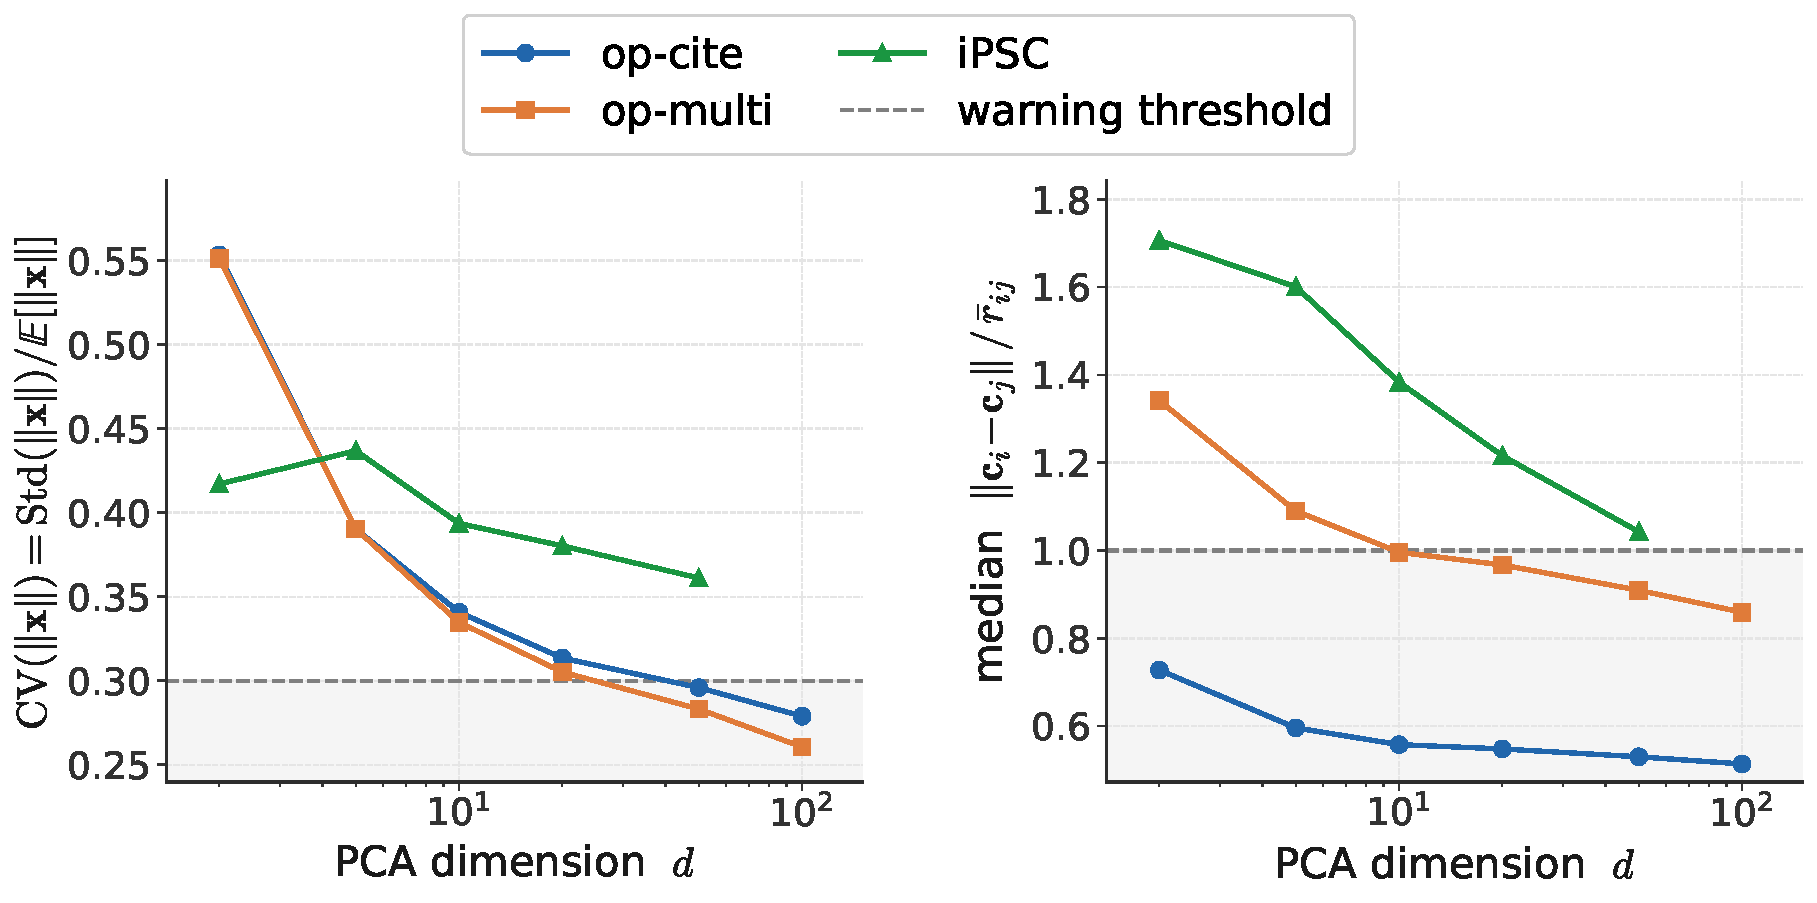
\includegraphics[width=\linewidth]{figures/norm_time_concentration_vs_dim.pdf}
        \vspace{-0.3em}
        % PAGECUT: caption compressed. Original: "High-dimensional concentration diagnostics. Dashed lines mark norm CV = 0.3 and inter-time/within-time ratio = 1.0."
        \captionof{figure}{High-dimensional concentration diagnostics. Dashed lines: norm CV $=0.3$, inter-time/within-time ratio $=1.0$.}
        \label{fig:norm-time-concentration-vs-dim}
    \end{minipage}\hfill
    \begin{minipage}[t]{0.54\linewidth} % PAGECUT: was 0.58\linewidth
        \centering
        \vspace{0pt}
        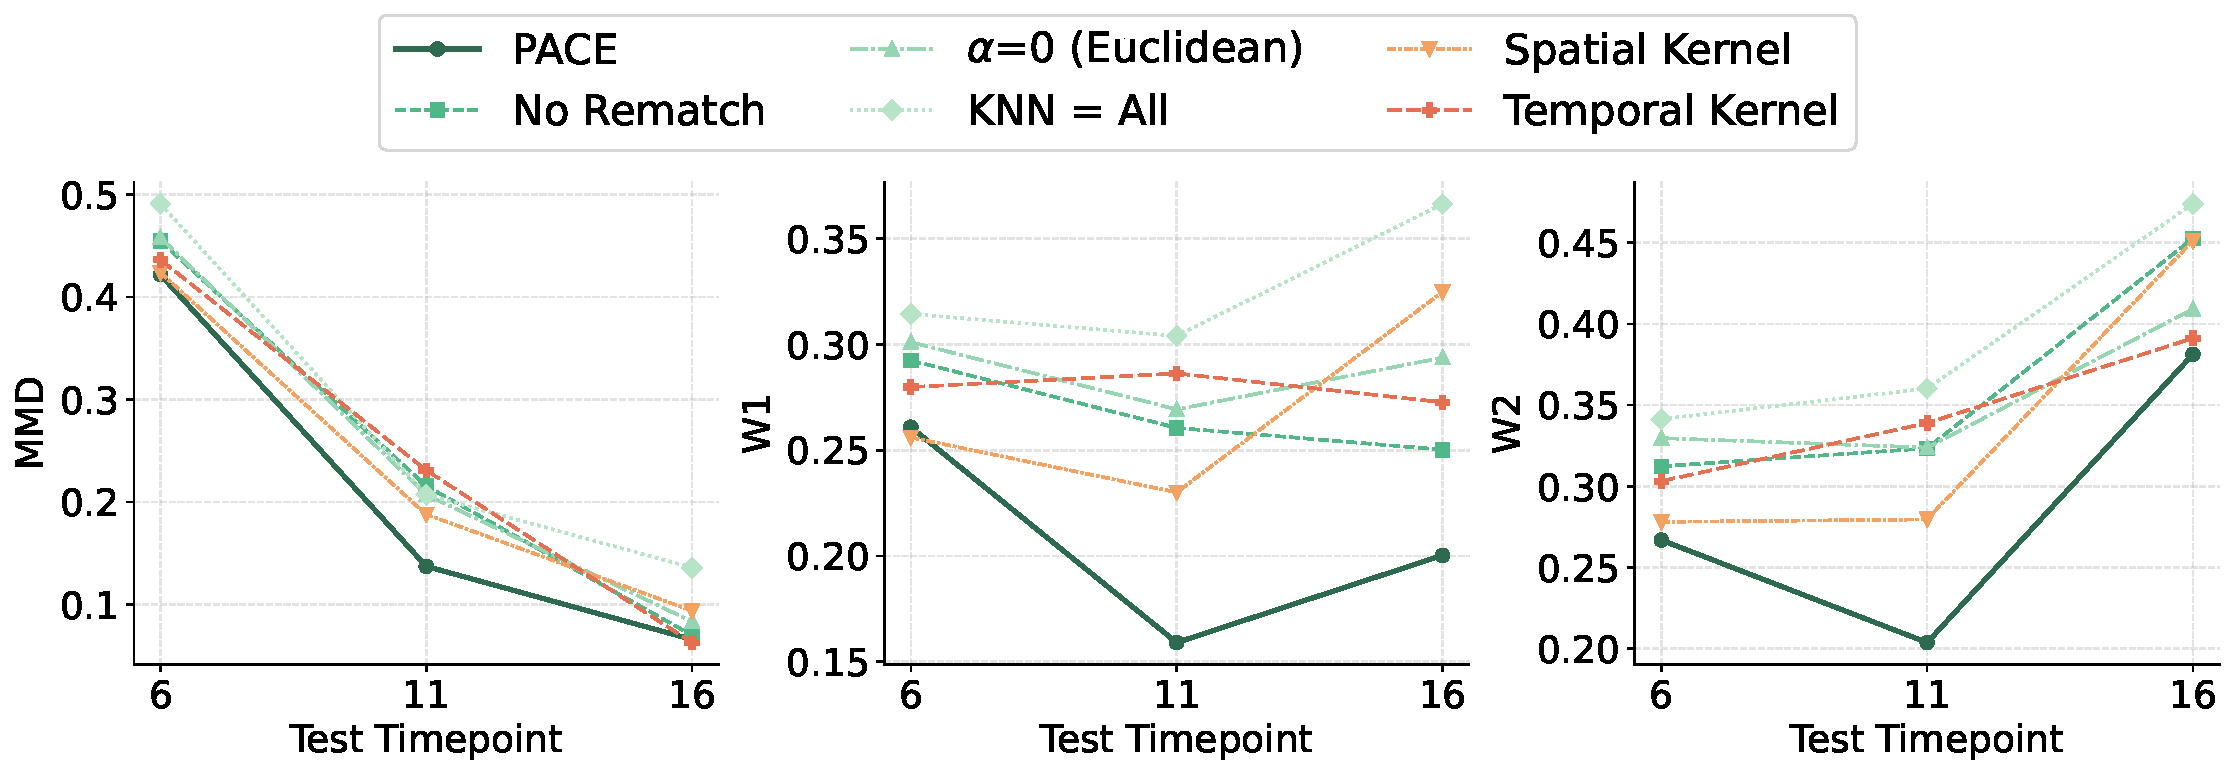
\includegraphics[width=\linewidth]{figures/pace_ablation_per_tp.pdf}
        \vspace{-0.3em}
        % PAGECUT: caption shortened; variant descriptions already appear in Sec.~4.5 text. Original:
        % "PACE ablations on Schiebinger2019 holdouts. Lower is better; variants remove rematching, use Euclidean action (alpha=0), use all neighbors, or drop spatial/temporal kernels."
        \captionof{figure}{PACE ablations on Schiebinger2019~\citep{schiebinger2019optimal} holdouts (lower is better).}
        \label{fig:pace-ablation-per-tp}
    \end{minipage}
\end{center}
